\chapter{Introduction}
\label{cha:intro}
\DIFaddbegin 

\chapquote{``As engineers, we would be foolish to ignore the lessons of a billion years of evolution.''}{Carver Mead}{1993}

%DIF > \begin{quotation}
%DIF > 	``As engineers, we would be foolish to ignore the lessons of a billion years of evolution.'' - Carver Mead, 1993
%DIF > \end{quotation}

\DIFaddend %Problem, motivation and significance
%TODO the origin of neuromorphic computing
%DIF < Neuromorphic computing has lead towards the development of biologically-inspired computer architectures 
Advances in computing power and machine learning have \DIFdelbegin \DIFdel{benefited computers with a rapid }\DIFdelend \DIFaddbegin \DIFadd{endowed computers with rapidly }\DIFaddend growing performance in cognitive tasks \DIFdelbegin \DIFdel{, }\DIFdelend such as recognising objects~\citep{deng2009imagenet} and playing GO~\citep{silver2016mastering}\DIFdelbegin \DIFdel{). 
These }\DIFdelend \DIFaddbegin \DIFadd{;
these }\DIFaddend tasks were once dominated by human intelligence and solved by biological neurons in the brain.
However, humans and many other animals still \DIFdelbegin \DIFdel{win against }\DIFdelend \DIFaddbegin \DIFadd{outperform }\DIFaddend computers in practical tasks, such as vision, and \DIFdelbegin \DIFdel{outperform }\DIFdelend in terms of size and energy cost \DIFdelbegin \DIFdel{over }\DIFdelend \DIFaddbegin \DIFadd{by }\DIFaddend several orders of magnitude.
For instance, AlphaGO~\citep{silver2016mastering} \DIFdelbegin \DIFdel{consumed }\DIFdelend \DIFaddbegin \DIFadd{has a power consumption of }\DIFaddend 1~MW \DIFdelbegin \DIFdel{of power on its 1920 }\DIFdelend \DIFaddbegin \DIFadd{on its $1,920$ }\DIFaddend CPUs and 280 GPUs when playing the game with one of the best human players whose brain \DIFdelbegin \DIFdel{only consumed about }\DIFdelend \DIFaddbegin \DIFadd{is rated at }\DIFaddend 20~W.
%DIF < Although we are still far from understanding the brain thoroughly, it is believed that the performance gap between computation in the biological nervous system and in a computer lies in the fundamental computing units and the way they act.
%DIF < Computers employ Boolean logic and deterministic digital operations based usually on synchronous clocks while nervous systems employ parallel-distributed, event-driven, stochastic unreliable components~\citep{indiveri2009artificial}.
%DIF < The impressive disparities in cognitive capabilities and energy consumption drives the research into biologically-inspired computers.
Although we are still far from understanding the brain thoroughly, it is believed that the performance gap between computation in the biological nervous system and in a computer lies in the \DIFaddbegin \DIFadd{nature of the }\DIFaddend fundamental computing units and how they compute.
Computers employ Boolean logic and deterministic digital operations \DIFdelbegin \DIFdel{based usually }\DIFdelend \DIFaddbegin \DIFadd{usually based }\DIFaddend on synchronous clocks while nervous systems employ \DIFdelbegin \DIFdel{parallel-distributed}\DIFdelend \DIFaddbegin \DIFadd{parallel, distributed}\DIFaddend , event-driven, stochastically unreliable components~\citep{indiveri2009artificial}\DIFdelbegin \DIFdel{, neurons.
The }\DIFdelend \DIFaddbegin \DIFadd{: neurons.
These }\DIFaddend impressive disparities in cognitive capabilities and energy consumption \DIFdelbegin \DIFdel{drives the }\DIFdelend \DIFaddbegin \DIFadd{drive }\DIFaddend research into biologically-plausible spiking neurons and brain inspired computers, known as \DIFdelbegin \DIFdel{neuromorphic engineering}\DIFdelend \DIFaddbegin \DIFadd{Neuromorphic Engineering}\DIFaddend ~(NE).
%DIF > Today	we	stand	poised	on	the	brink	of	a	new	era	of	compu:ng	in	which	technology	is	more	
%DIF > consumable,	insight-driven	and	cogni:ve.	IBM	Research	is	exploring	and	developing	the	
%DIF > enabling	technologies	that	will	transform	the	way	computers	are	used	
%DIF > Ginni	Rome]y	
%DIF > IBM	President,	Chairman	and	CEO	




\DIFdelbegin %DIFDELCMD < \begin{figure}[tbh!]
%DIFDELCMD < 	\centering
%DIFDELCMD < 	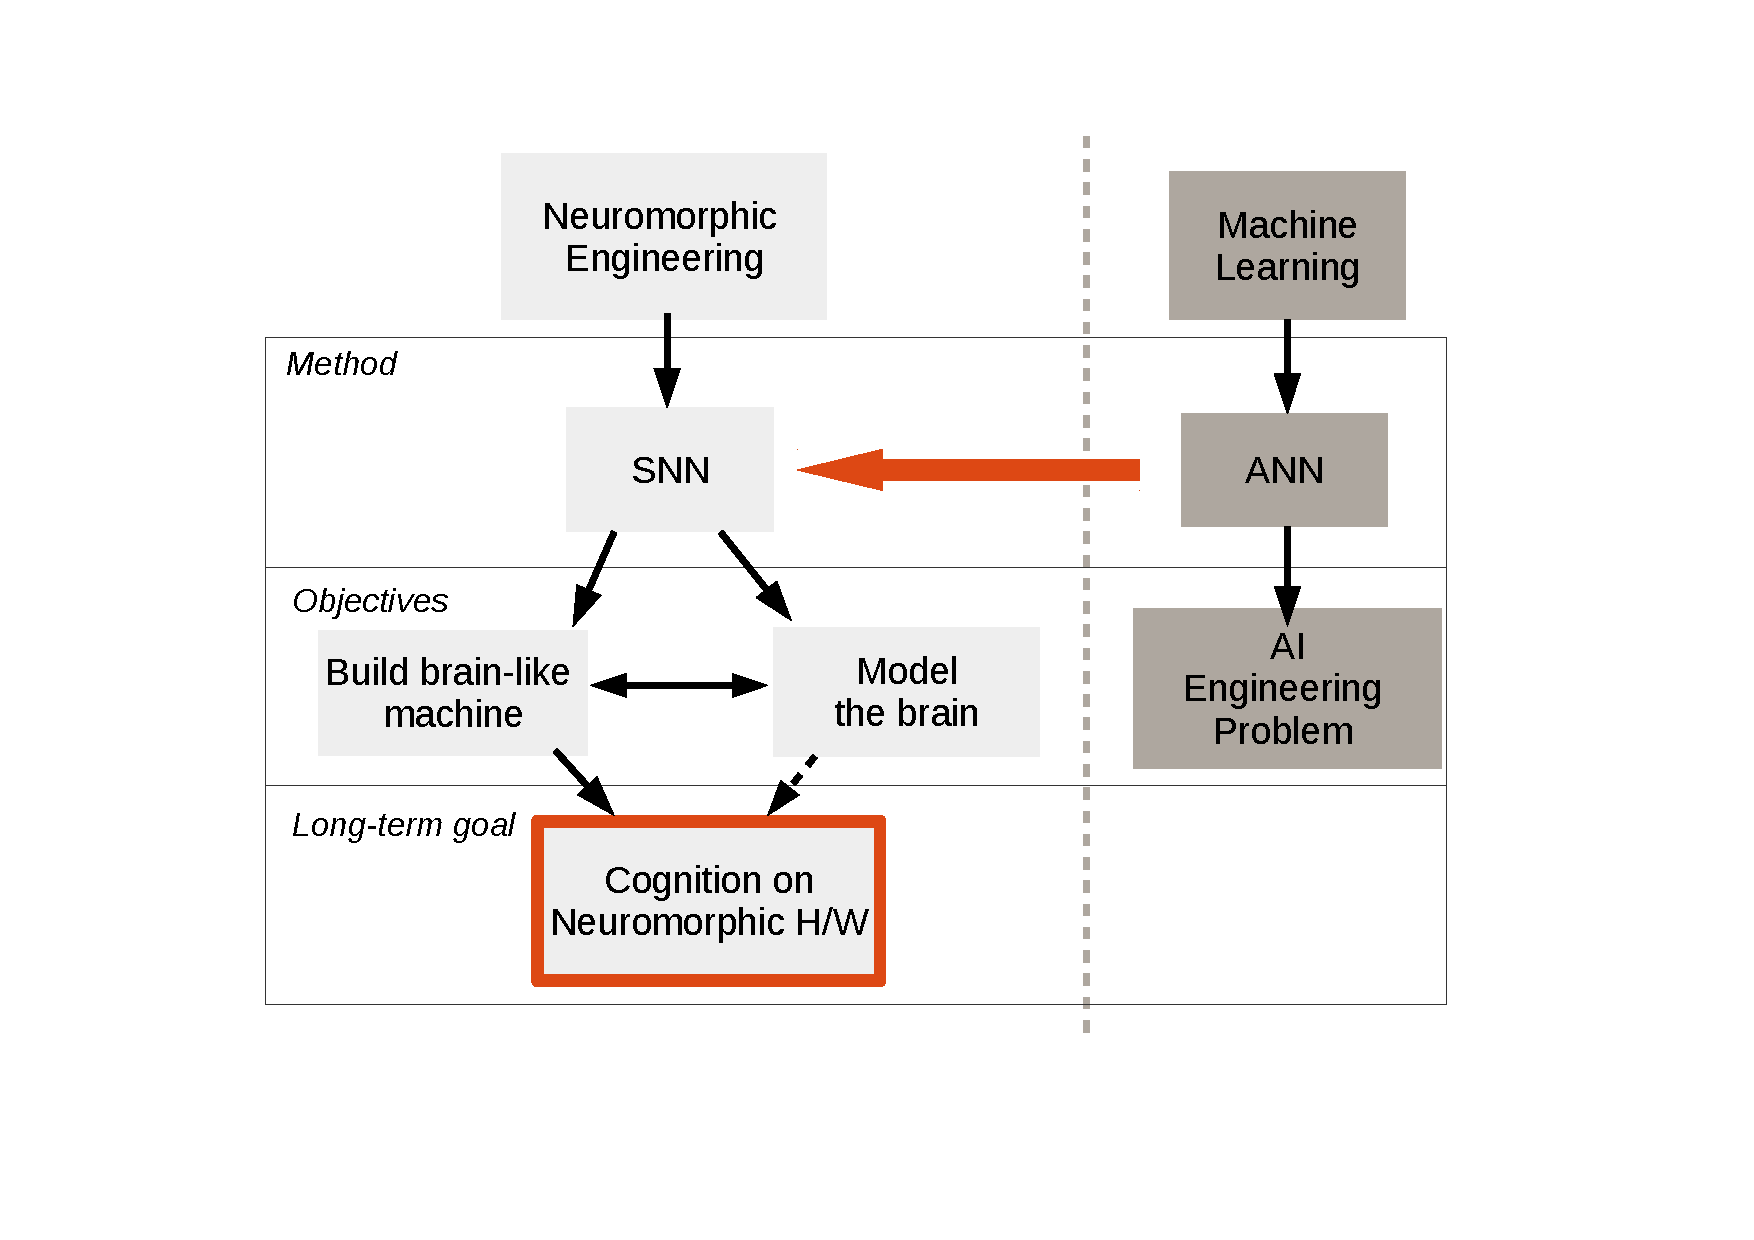
\includegraphics[width=1.0\textwidth]{pics_intro/intro2.pdf}
%DIFDELCMD < 	%%%
%DIFDELCMD < \caption{%
{%DIFAUXCMD
\DIFdel{
		The outline of the problem statement of the work.
%DIF < 		Neuromorphic engineering and machine learning has been diverging.
%DIF < 		This thesis merge the objectives to the ultimate goal of cognition on neuromorphic hardware.
		}}
	%DIFAUXCMD
%DIFDELCMD < \label{fig:intro}
%DIFDELCMD < \end{figure}
%DIFDELCMD < %%%
%DIF < which may alternate conventional Von Neumann and rival the Human brain in terms of energy efficiency and cognitive capabilities.
\DIFdelend %Two aims
NE was proposed by Carver Mead in the late 1980s \citep{Mead:1989:AVN:64998} to build analogue circuits \DIFdelbegin \DIFdel{that mimic the }\DIFdelend \DIFaddbegin \DIFadd{which mimic }\DIFaddend biological neural cells and the architecture of the nervous system using \DIFdelbegin \DIFdel{very-large-scale integration }\DIFdelend \DIFaddbegin \DIFadd{Very-Large-Scale Integration }\DIFaddend (VLSI) technology.
%DIF < ``As engineers, we would be foolish to ignore the lessons of a billion years of evolution.''
\DIFdelbegin \DIFdel{Figure~\ref{fig:intro} indicates }\DIFdelend \DIFaddbegin \DIFadd{With the ultimate goal of equipping neuromorphic machines with genuine intelligence, 
%DIF > ~\citep{konar1999artificial}, also known as `Neuromorphic Cognition'~\citep{indiveri2009artificial},
}\DIFaddend the objectives of NE \DIFaddbegin \DIFadd{can be summarised as follows}\DIFaddend ~\citep{furber2007neural}:
\begin{itemize}
	\item \DIFdelbegin \DIFdel{neuromorphic }\DIFdelend \DIFaddbegin \DIFadd{brain }\DIFaddend modelling: for neuroscientists to understand the brain by modelling and simulating the activities of \DIFdelbegin \DIFdel{the }\DIFdelend biological neurons; 
	\item neuromorphic computing: for engineers to build brain-like machines by applying biological \DIFdelbegin \DIFdel{features }\DIFdelend \DIFaddbegin \DIFadd{principles }\DIFaddend to computers.
\end{itemize}
\DIFdelbegin \DIFdel{This is a bidirectional process that }\DIFdelend \DIFaddbegin \DIFadd{The aims complement each other; }\DIFaddend building a biologically inspired computer requires a better understanding of the brain, and simulating brain activities at large scale and in real time \DIFdelbegin \DIFdel{can be only feasible }\DIFdelend \DIFaddbegin \DIFadd{is feasible only }\DIFaddend on massively-parallel neuromorphic hardware.



\DIFdelbegin \DIFdel{Since around 2004 to 2005, `Dennard's Law' has no longer been followed~\mbox{%DIFAUXCMD
\citep{bohr200730}
}%DIFAUXCMD
, so as transistors get smaller their power density no longer stays constant but starts to increase.
The breakdown of Dennard scaling and the problem of power dissipation drove chip manufacturers to multi/many-core architecture.
However, the increased number of active transistors in a multi-core chip costs more power consumption thus creating the prospect that some fraction of the cores will have to remain completely powered-off given the thermal design power constraint.
Dark silicon~\mbox{%DIFAUXCMD
\citep{esmaeilzadeh2011dark}
}%DIFAUXCMD
addresses the issue of inactive areas of a multi-core chip, which could be 50}%DIFDELCMD < \% %%%
\DIFdel{of nodes in an 8~nm technology.
Neuromorphic engineering offers a potential solution for power dissipation by applying the biological features of event-driven, hybrid analogue/digital, unreliable components to computers.
Moreover, most of the neural interconnections in the brain are local, and the `memory' units attach to the `computation' node in a neuron.
Therefore, learning from biology may give computers an alternative to the conventional Von Neumann architecture and thus may solve the problem of the microprocessor/memory performance gap~\mbox{%DIFAUXCMD
\citep{wulf1995hitting}
}%DIFAUXCMD
, also known as the Von Neumann bottleneck, where the system speed is determined and limited by the memory performance.
}%DIFDELCMD < 

%DIFDELCMD < %%%
%DIF < SNN
\DIFdelend %DIF > Since around 2004 to 2005, `Dennard's Law' has no longer been followed~\citep{bohr200730}, so as transistors get smaller their power density no longer stays constant but starts to increase.
%DIF > The breakdown of Dennard scaling and the problem of power dissipation drove chip manufacturers to multi/many-core architecture.
%DIF > However, the increased number of active transistors in a multi-core chip costs more power consumption thus creating the prospect that some fraction of the cores will have to remain completely powered-off given the thermal design power constraint.
%DIF > Dark silicon~\citep{esmaeilzadeh2011dark} addresses the issue of inactive areas of a multi-core chip, which could be 50\% of nodes in an 8~nm technology.
%DIF > Neuromorphic engineering offers a potential solution for power dissipation by applying the biological features of event-driven, hybrid analogue/digital, unreliable components to computers.
%DIF > Moreover, most of the neural interconnections in the brain are local, and the `memory' units attach to the `computation' node in a neuron.
%DIF > Therefore, learning from biology may give computers an alternative to the conventional Von Neumann architecture and thus may solve the problem of the microprocessor/memory performance gap~\citep{wulf1995hitting}, also known as the Von Neumann bottleneck, where the system speed is determined and limited by the memory performance.

%DIF < Although there are a number of neuromorphic platforms available for large-scale SNN simulations,
\DIFdelbegin \DIFdel{During the last decade, researchers have used the capabilities created by rapid developments in neuromorphic engineering }\DIFdelend %DIF > Why SNN
\DIFaddbegin \DIFadd{Spiking Neural Networks (SNNs), comprised of spiking neurons, hold the key }\DIFaddend to address the dual aims of understanding brain functions and building brain-like machines.
\DIFdelbegin \DIFdel{Spiking Neural Networks (SNN) hold the key as the main approach for both goals.
The so-called third generation of artificial neural network (ANN)~\mbox{%DIFAUXCMD
\citep{maass1997networks}
}%DIFAUXCMD
introduces biological realism to neural modelling.
}\DIFdelend The spiking neuron mathematically models the dynamics of a single neuron \DIFaddbegin \DIFadd{with biological realism }\DIFaddend and the network describes the architecture of the neural connections and the information transmission among them\DIFdelbegin \DIFdel{.
Neuroscientists }\DIFdelend \DIFaddbegin \DIFadd{; readers can refer to Chapter~\ref{cha:bkg} for more detail.
Therefore, neuroscientists are able to }\DIFaddend reproduce the recorded neural dynamics and activities from \textit{in-vivo/vitro} experiments to verify their models and measure the progress of brain understanding,
\DIFdelbegin \DIFdel{While computer engineers }\DIFdelend \DIFaddbegin \DIFadd{while computer engineers can }\DIFaddend focus on the hardware implementations of the \DIFdelbegin \DIFdel{SNN models.
Hence, SNN simulation tools~\mbox{%DIFAUXCMD
\citep{davison2008pynn, gewaltig2007nest, goodman2008brian}
}%DIFAUXCMD
and neuromorphic hardware platforms~\mbox{%DIFAUXCMD
\citep{furber2014spinnaker,  schemmel2010wafer,benjamin2014neurogrid,merolla2014million}
}%DIFAUXCMD
have been developed to allow exploration of the brainby mimicking its functions and developing large-scale practical applications~\mbox{%DIFAUXCMD
\citep{eliasmith2012large}
}%DIFAUXCMD
.
In addition, neuromorphic engineering has delivered biologically-inspired sensors such as DVS~(Dynamic Vision Sensor) silicon retinas~\mbox{%DIFAUXCMD
\citep{serrano2013128, delbruck2008frame, yang2015dynamic, posch2014retinomorphic}
}%DIFAUXCMD
, and DAS~(Dynamic Audition Sensor)~\mbox{%DIFAUXCMD
\citep{5537164}
}%DIFAUXCMD
, which offer the prospect of low-cost sensory processing thanks to their event-driven and redundancy-reducing style of information representation.
}\DIFdelend \DIFaddbegin \DIFadd{spiking neurons and the interconnections between them to build energy-efficient neuromorphic hardware.
}\DIFaddend 

%DIF < how to operate these brain-like machines to be competent in cognitive applications still remains unsolved.
\DIFdelbegin \DIFdel{The long-term ultimate goal of NE is to equip neuromorphic machines with genuine intelligence~\mbox{%DIFAUXCMD
\citep{konar1999artificial}
}%DIFAUXCMD
.
Today, in neuromorphic modelling, we know that information processing in the brain is conducted by the basic computing units, the spiking neurons.Information transmission takes place in the synapses andwe can draw the connections among neurons from anatomical experiments.
In neuromorphic computing, massive large-scale SNN hardware simulators are ready to use.
However, due to }\DIFdelend \DIFaddbegin \DIFadd{Over the last decade, considerable development has taken place in NE where simulations of massive SNNs~\mbox{%DIFAUXCMD
\citep{markram2006blue,ananthanarayanan2009cat}
}%DIFAUXCMD
have proved to be significantly useful in understanding the brain, and large-scale neuromorphic platforms have been launched to simulate SNNs in hardware.
%DIF > , such as the High Input Count Analog Neural Network (HI-CANN)~\citep{schemmel2010wafer}, Neurogrid~\citep{benjamin2014neurogrid}, SpiNNaker~\citep{furber2014spinnaker}, TrueNorth~\citep{merolla2014million}, and HiAER-IFAT~\citep{yu201265k}.
These neuromorphic computers develop into energy-efficient systems by implementing neurons, synapses and neuronal communications on analogue circuits~\mbox{%DIFAUXCMD
\citep{schemmel2010wafer,benjamin2014neurogrid,yu201265k}
}%DIFAUXCMD
or exploiting parallel low-power microprocessors on digital hardware~\mbox{%DIFAUXCMD
\citep{furber2014spinnaker,merolla2014million}
}%DIFAUXCMD
. 
%DIF > Some of these neuromorphic computers~\citep{schemmel2010wafer,benjamin2014neurogrid,merolla2014million} use non-Von Neumann architectures to mimic the characteristics of parallelism, scalability, and fault-tolerance of the neural system.
%DIF > Instead of executing sequential instructions and building systems of separated computing and memory units, they rather copy the nature of the brain; implementing neurons, synapses and neuronal communications on analogue/digital microelectronics.
%DIF > Therefore this novel architecture may solve the problem of the microprocessor/memory performance gap~\citep{wulf1995hitting}, also known as the Von Neumann bottleneck, where the system speed is determined and limited by the memory performance;
%DIF > and at the same time, these neuromorphic computers develop into energy-efficient systems by reducing the energy used for data movement between processors and memories, and by employing event-based computing. 
Thus, }\DIFaddend the \DIFdelbegin \DIFdel{fundamental difference of data representation and neural computation between spiking and artificial neurons , how to operate these brain-like }\DIFdelend \DIFaddbegin \DIFadd{neuromorphic hardware systems composed with those have successfully demonstrated decreased energy cost of SNN simulations on supercomputers~\mbox{%DIFAUXCMD
\citep{de2010world,sharp2012power}
}%DIFAUXCMD
.
}

\DIFadd{However, the SNN simulations only reconstruct the network behaviours and neural dynamics of some subsystem of the brain, `but without precisely functionally simulating that subsystem'~\mbox{%DIFAUXCMD
\citep{de2010world}
}%DIFAUXCMD
.
Therefore, this type of SNN simulation can be used to guide neuroscience and the development of neuromorphic hardware systems, but is not directly useful for solving cognitive tasks.
Recent SNN applications~\mbox{%DIFAUXCMD
\citep{bill2014compound,diehl2015unsupervised}
}%DIFAUXCMD
in Artificial Intelligence~(AI) tasks, summarised in Chapter~\ref{cha:bench}, typically comprise only two neural layers and exploit biologically-plausible learning rules, e.g. Spike-Timing-Dependent Plasticity (STDP), and/or Winner-Take-All~(WTA) circuits on the synaptic connections.
These two-layered SNN models are considered to be `reactive' since the output neurons simply react to the sensory input.
Consequently, such SNNs cannot perform sophisticated effective cognition as can the brain;
thus programming these neuromorphic }\DIFaddend machines to be competent in cognitive applications still remains unsolved.
\DIFaddbegin \DIFadd{\mbox{%DIFAUXCMD
\citet{indiveri2009artificial}
}%DIFAUXCMD
argued that the next substantial challenge of NE is to make these brain-like computers effectively cognitive, also known as `Neuromorphic Cognition'.
%DIF > such that SNNs have not been widely used in Artificial Intelligence~(AI) engineering problems.
%DIF > Therefore, \citet{indiveri2009artificial} argued that towards the ultimate goal of genuine intelligence on neuromorphic hardware, the next significant challenge of NE is to enable these brain-inspired computers to solve cognitive tasks, also known as `Neuromorphic Cognition'.
}\DIFaddend 


%DIF > Today, however, NE stands before a large con-
%DIF > ceptual challenge that must be met before there will be
%DIF > significant progress toward an age of genuinely intelligent
%DIF > neuromorphic machines. The challenge is to bridge the gap
%DIF > from reactive systems to ones that are cognitive in quality.
%DIF > In NE, as in neuroscience and computer science, we
%DIF > understand very little about how to configure these large
%DIF > systems to achieve the sophistication of processing that we
%DIF > could regard as effective cognition.
%DIF > 
%DIF > In the case of NE and neuroscience, the question is
%DIF > sharpened by the need to understand cognition in the
%DIF > context of the nervous systems’ peculiar hardware and
%DIF > style of processing. We know, for instance, that nervous
%DIF > systems can exhibit context-dependent behavior, can exe-
%DIF > cute ‘‘programs’’ consisting of series of flexible steps, and
%DIF > can conditionally branch to alternative behaviors, using
%DIF > spiking neurons and dynamic synapses as basic computa-
%DIF > tional modules.
%DIF > 
%DIF > The NE community has recently developed efficient
%DIF > VLSI implementations of such types of computational
%DIF > modules: next to several designs of conductance-based and
%DIF > integrate-and-fire neurons [19, 25, 38, 58, 66], NE
%DIF > researchers proposed circuits that implement VLSI
%DIF > dynamic synapses [7], spike-based plasticity mechanisms
%DIF > [32, 34, 50, 68], and soft winner-take-all (WTA) networks
%DIF > [16], for example.VLSI implementations of WTA networks
%DIF > of spiking neurons, with plastic dynamic synapse circuits
%DIF > are particularly important, because recent theoretical
%DIF > studies demonstrated that recurrent neural networks
%DIF > arranged in a way to implement soft WTA performance can
\DIFaddbegin 

%DIF > Meanwhile, Deep Learning research in the field of Artificial Neural Network~(ANN) has dominated state-of-the-art solutions for AI engineering tasks, e.g. exceeding human-level performance on image classification~\citep{he2015delving}, see Chapter~\ref{cha:dnn} for more examples.
\DIFadd{STDP as a learning mechanism based on biological observations has been theoretically proved to be equivalent to a stochastic version of powerful machine learning algorithms, such as Expectation Maximisation~\mbox{%DIFAUXCMD
\citep{nessler2013bayesian}
}%DIFAUXCMD
, Contrastive Divergence~\mbox{%DIFAUXCMD
\citep{neftci2013event}
}%DIFAUXCMD
, Markov Chain Monte Carlo \mbox{%DIFAUXCMD
\citep{buesing2011neural}
}%DIFAUXCMD
and Gradient Descent~\mbox{%DIFAUXCMD
\citep{o2016deep}
}%DIFAUXCMD
.
However, in practice, there have been two significant problems prohibiting the SNN from becoming as `intelligent' as its non-spiking counterpart, the Artificial Neural Network~(ANN).
Firstly, }\DIFaddend Deep Learning research \DIFaddbegin \DIFadd{has made great achievements }\DIFaddend in the field of ANNs \DIFdelbegin \DIFdel{has dominated the }\DIFdelend \DIFaddbegin \DIFadd{and dominated }\DIFaddend state-of-the-art solutions \DIFdelbegin \DIFdel{on cognitive }\DIFdelend \DIFaddbegin \DIFadd{for AI engineering }\DIFaddend tasks, e.g. \DIFdelbegin \DIFdel{the }\DIFdelend exceeding human-level performance on image classification\DIFdelbegin \DIFdel{tasks~\mbox{%DIFAUXCMD
\citep{he2015delving}
}%DIFAUXCMD
.
Figure~\ref{fig:intro} shows the diverging objectives of SNNs and ANNs, where SNNs focus on mimicking the brain while ANNs are active in solving engineering AI problems.
%DIF < TODO need to modify
Despite remarkable computational success, ANNs ignore the spiking nature of neural communication that is fundamental for biological neuronal networks.
At the same time, }\DIFdelend \DIFaddbegin \DIFadd{~\mbox{%DIFAUXCMD
\citep{he2015delving}
}%DIFAUXCMD
, see Chapter~\ref{cha:dnn} for more examples.
However, the fundamental differences in data representation and neural computation between spiking and artificial neurons make it difficult to transform ANN models into SNN algorithms, see Chapter~\ref{cha:bkg} for more detail.
Secondly, the computation cost for simulating large SNNs of size comparable to commonly-used deep ANNs was considered to be infeasible, though this has gradually been solved by NE.
%DIF > Thus, recent SNN applications~\citep{bill2014compound,diehl2015unsupervised} in AI tasks (summarised in Chapter~\ref{cha:bench}) typically comprise only two neural layers and exploit STDP learning rules and/or Winner-Take-All~(WTA) circuits on the synaptic connections.
%DIF > These models are `reactive' systems since the output neurons simply react to the sensory input.
%DIF > Therefore, such SNNs cannot perform sophisticated effective cognition as can deep ANNs.
}

%DIF > These models are `reactive' since they typically comprise only two neural layers, where the output neurons simply react to the input.
%DIF > Therefore, such SNNs cannot perform sophisticated effective cognition as can deep ANNs.
%DIF > Meanwhile, Deep Learning research in the field of artificial neural networks~(ANNs) has dominated state-of-the-art solutions for AI engineering tasks, e.g. exceeding human-level performance on image classification~\citep{he2015delving}, see Chapter~\ref{cha:dnn} for more examples.
%DIF > Although theoretical studies have shown that biologically-plausible learning, e.g. Spike-Timing-Dependent Plasticity~(STDP), could approximate a stochastic version of powerful machine learning algorithms, such as Expectation Maximization~\citep{nessler2013bayesian}, Contrastive Divergence~\citep{neftci2013event}, Markov Chain Monte Carlo \citep{buesing2011neural} and Gradient Descent~\citep{o2016deep},
%DIF > %Stochasticity, in contrast with the continuously differentiable functions used by ANNs, is intrinsic to the event-based spiking process, making network training difficult.
%DIF > in practice, there have been two significant problems prohibiting the SNN from becoming as `intelligent' as its non-spiking counterpart, the ANN.
%DIF > Firstly, the fundamental differences in data representation and neural computation between spiking and artificial neurons make it difficult to transform ANN models to SNN algorithms, see Chapter~\ref{cha:bkg} for more detail.
%DIF > %Therefore it is relative easy to build SNN models and observe their dynamics for use in neuroscience, but much harder to construct SNNs with biological realism and specific functions for AI applications.
%DIF > Secondly, the computation cost for simulating large SNNs of size comparable to commonly-used deep ANNs was considered to be infeasible, but has been gradually solved by NE.
%DIF > Chapter~\ref{cha:bench} summarises recent developments in applying SNNs in AI tasks, where these SNN models perform as `reactive' systems and exploit Winner-Take-All~(WTA) circuits and spike-based plasticity~\citep{bill2014compound,diehl2015unsupervised}.
%DIF > These models are `reactive' since they typically comprise only two neural layers, where the output neurons simply react to the input.
%DIF > Therefore, such SNNs cannot perform sophisticated effective cognition as can deep ANNs.


%DIF > Therefore, with neuromorphic hardware ready, the increasing knowledge of SNNs and the success of Deep Learning in ANNs, it is time to take an extra step towards the ultimate goal of NE by equipping neuromorphic computers with equivalent performance as ANNs' to solve AI engineering tasks.
%DIF > 
%DIF > %However, the SNN has not achieved the performance of its non-spiking counterpart, the ANN, in cognitive tasks particularly when used in deep neural networks.
%DIF > %%TODO Current status

%DIF > Meanwhile, Deep Learning research in the field of ANNs has dominated state-of-the-art solutions for AI engineering tasks, e.g. exceeding human-level performance on image classification~\citep{he2015delving}, see Chapter~\ref{cha:dnn} for more examples.

%DIF > With neuromorphic hardware ready for massive SNN simulations, the main research problem arises: how to improve the cognitive performance of SNNs to catch up with that of ANNs.

\DIFadd{With the neuromorphic platforms ready for massive SNN simulations, this, therefore, is the main research problem: to improve the cognitive performance of SNNs }\DIFaddend to catch up with \DIFdelbegin \DIFdel{ANNs' ability to beat human performance using SNNs , a shared ultimate goal has emerged.
The key problem of the research describe in this thesis is to enable SNNs to have cognitive capabilities, and the main challenge is to close the gap of }\DIFdelend \DIFaddbegin \DIFadd{that of ANNs.
Hence, researchers turn to Deep Learning to build `smarter' SNNs.
Initial studies have shown that SNNs can be trained by first training an equivalent deep ANN and then transferring the tuned weights to the SNN;
this method is called `off-line' training, since it does not take place on SNNs directly, but rather on ANNs instead.
Chapter~\ref{cha:Conv} discusses these `off-line' training models in detail, and proposes a simple, generalised, off-line SNN training method to overcome the problems of poor modelling accuracy and high computational complexity of the existing methods~\mbox{%DIFAUXCMD
\citep{Jug_etal_2012,hunsberger2015spiking,diehl2015fast}
}%DIFAUXCMD
.
To embed the biologically-plausible learning rules into deep SNN training, researchers take an extra step to `on-line' methods where Deep Learning modules can be trained purely on SNNs in an event-driven manner, see Chapter~\ref{cha:sdlm}.
Previous work~\mbox{%DIFAUXCMD
\citep{neil2013online,neftci2013event,burbank2015mirrored}
}%DIFAUXCMD
has failed to provide SNNs with recognition accuracy equivalent to ANNs due to }\DIFaddend the \DIFdelbegin \DIFdel{cognition performance of SNNs and ANNs.
}\DIFdelend \DIFaddbegin \DIFadd{lack of mathematical analysis.
We continue the inspiring work on these biologically-plausible `on-line' training methods and propose a formalised method to train multi-layered Deep Learning modules on SNNs.
}\DIFaddend 

%DIF < TODO Why it motivates me (why it would be useful and important to have a solution)
\DIFaddbegin \DIFadd{To provide meaningful comparisons between these proposed SNN models and other existing methods within the rapidly advancing field of NE, we propose a large dataset of spike-based visual stimuli and a corresponding evaluation methodology to estimate the overall performance of SNN models and their hardware implementations in Chapter~\ref{cha:bench}.
}\DIFaddend 

\section{\DIFdelbegin \DIFdel{Statement of the Problem}\DIFdelend \DIFaddbegin \DIFadd{Motivation and Aims}\DIFaddend }
%DIF > \section{Statement of the Problem}
\label{sec:state_problem}
NE has led to the development of biologically-inspired computer architectures which may \DIFdelbegin \DIFdel{provide an alternative to the conventional Von Neumann architecture and achieve }\DIFdelend \DIFaddbegin \DIFadd{approach }\DIFaddend the performance of \DIFaddbegin \DIFadd{the }\DIFaddend human brain in terms of energy efficiency and cognitive capabilities.
%DIF >  provide an alternative to the conventional Von Neumann architecture and 
Although there are a number of neuromorphic platforms available for large-scale \DIFdelbegin \DIFdel{SNN simulations, }\DIFdelend \DIFaddbegin \DIFadd{Spiking Neural Network~(SNN) simulations, the problem of }\DIFaddend programming these brain-like machines to be competent in cognitive applications still remains unsolved.
On the other hand\DIFaddbegin \DIFadd{, }\DIFaddend Deep Learning has emerged in \DIFdelbegin \DIFdel{ANN }\DIFdelend \DIFaddbegin \DIFadd{Artificial Neural Network (ANN) }\DIFaddend research to dominate state-of-the-art solutions for cognitive tasks.
Thus \DIFdelbegin \DIFdel{it raises }\DIFdelend the main research problem \DIFdelbegin \DIFdel{of }\DIFdelend \DIFaddbegin \DIFadd{emerges of understanding }\DIFaddend how to operate and train \DIFdelbegin \DIFdel{networks of }\DIFdelend biologically-plausible \DIFdelbegin \DIFdel{spiking neurons }\DIFdelend \DIFaddbegin \DIFadd{SNNs }\DIFaddend to close the gap \DIFdelbegin \DIFdel{of }\DIFdelend \DIFaddbegin \DIFadd{in }\DIFaddend cognitive capabilities between SNNs and ANNs \DIFdelbegin \DIFdel{in AI tasks?
}\DIFdelend \DIFaddbegin \DIFadd{on AI tasks.
}\DIFaddend 

%DIF < Although training SNNs in general is believed to be difficult,  combining deep learning with spiking neurons thus to train SNNs of deep architectures can be simple, effective and generalised because existing approaches have shown promising results in the early stage of the study.
%DIF > TODO Why it motivates me (why it would be useful and important to have a solution)
%DIF > This thesis aims to provide the NE community with generalised SNN training methods and performance evaluation methodologies

\DIFdelbegin \section{\DIFdel{Hypotheses and Aims}}
%DIFAUXCMD
\addtocounter{section}{-1}%DIFAUXCMD
%DIFDELCMD < \label{sec:aim}
%DIFDELCMD < %%%
%DIF < The main objective is to improve the cognitive capability of SNNs and equip them with the equivalent learning ability of ANNs for AI applications.
%DIF < %In addition, to run such a biologically-plausible model on a complete hardware platform validates the feasibility of real-time Neuromorphic Computing for cognitive tasks.
%DIF < Moreover, it is necessary to provide the community with a uniform dataset and an evaluation methodology to compare the performance of SNN models and hardware platforms.
%DIF < The goals at this ????? to show that: 
\DIFdelend \DIFaddbegin \DIFadd{Enabling this massively-parallel neuromorphic hardware to deliver state-of-the-art performance on AI tasks will be a big step towards Neuromorphic Cognition.
It will contribute to the ultimate goal of equipping brain-inspired computers with Human brain levels of energy efficiency and cognitive capability. 
}\DIFaddend 


\DIFaddbegin \section{\DIFadd{Thesis Statement and Hypotheses}}
\label{sec:aim}
\DIFaddend Although fundamental differences \DIFdelbegin \DIFdel{on }\DIFdelend \DIFaddbegin \DIFadd{in }\DIFaddend input/output representation and neural computation exist between spiking and conventional artificial neurons, the cognitive capability of SNNs can be improved to catch up with \DIFdelbegin \DIFdel{the ANNs ' by embedding deep learning }\DIFdelend \DIFaddbegin \DIFadd{that of ANNs by embedding Deep Learning }\DIFaddend techniques in training SNNs\DIFdelbegin \DIFdel{, because deep learning has }\DIFdelend \DIFaddbegin \DIFadd{.
Deep Learning has not only }\DIFaddend successfully equipped ANNs with better-than-human performance on AI tasks\DIFdelbegin \DIFdel{and inspiring works have been reported in training }\DIFdelend \DIFaddbegin \DIFadd{, but also theoretical studies have proved the equivalent learning capability of SNNs, and neuromorphic hardware is ready for operating large-scale }\DIFaddend deep SNNs.
\DIFdelbegin \DIFdel{Accordingly}\DIFdelend \DIFaddbegin 

\DIFadd{According to the thesis statement}\DIFaddend , the hypotheses \DIFdelbegin \DIFdel{and equivalent goals at this thesis are }\DIFdelend \DIFaddbegin \DIFadd{are defined }\DIFaddend as follows: 
\begin{itemize}
%	\item 
%	An object recognition system can operate in real-time on a complete neuromorphic platform in an absolute spike-based fashion.
%	The hypothesis paves the way for further study with solid proof of the capability of real-time cognitive application built on neuromorphic platform.
%
%	Aim: to build a real-time neuromorphic object recognition prototype running on hardware SNN simulator and receiving visual input from a DVS sensor.

	\item 
%	SNNs can deliver equivalent cognitive capability to conventional ANNs for object recognition applications.
	Deep SNNs can be successfully and simply trained off-line where the training takes place on equivalent ANNs and \DIFdelbegin \DIFdel{then transferring the trained weights back to }\DIFdelend \DIFaddbegin \DIFadd{the tuned weights then transferred back to the }\DIFaddend SNNs, thus \DIFdelbegin \DIFdel{to make }\DIFdelend \DIFaddbegin \DIFadd{making }\DIFaddend them as competent as ANNs in cognitive tasks.

\DIFdelbegin \DIFdel{Aim: to generalise a training method on conventional ANNs whose trained connections can be transferred to corresponding SNNs with close recognition performance.
}\DIFdelend %DIF > 	Aim: to generalise a training method on conventional ANNs whose trained connections can be transferred to corresponding SNNs to deliver similar recognition performance.

	\item 
	Unsupervised Deep Learning modules can be trained on-line on SNNs with biologically-plausible synaptic plasticity to demonstrate a learning capability as competent as ANNs.

\DIFdelbegin \DIFdel{Aim: to formalise a local learning rule based on synaptic plasticity for unsupervised, event-based, biologically-plausible training of deep SNNs in order to catch up the recognition performances of ANNs.
}\DIFdelend %DIF > 	Aim: to formalise a local learning rule based on synaptic plasticity for unsupervised, event-based, biologically-plausible training of deep SNNs in order to catch up with the recognition performances of ANNs.

	\item 
	A new set of spike-based vision datasets can provide resources \DIFdelbegin \DIFdel{to support fair competition between researchers since new concerns relating to energy efficiency and recognition latency emerge in Neuromorphic Vision.
}%DIFDELCMD < 

%DIFDELCMD < 	%%%
\DIFdel{Aim: to provide a unified spiking version of a commonly-used dataset and a complementary }\DIFdelend \DIFaddbegin \DIFadd{and corresponding }\DIFaddend evaluation methodology to \DIFdelbegin \DIFdel{assess the performance of SNN algorithms.
}\DIFdelend \DIFaddbegin \DIFadd{support objective comparisons and measure progress within the rapidly advancing field of NE.
}

%DIF > 	Aim: to provide a unified spiking version of a commonly-used dataset and a complementary evaluation methodology to assess the performance of SNN algorithms.
\DIFaddend \end{itemize}


\section{Contributions}
The primary \DIFdelbegin \DIFdel{achievements }\DIFdelend \DIFaddbegin \DIFadd{achievement }\DIFaddend of the work described in this thesis \DIFdelbegin \DIFdel{are }\DIFdelend \DIFaddbegin \DIFadd{is }\DIFaddend the training of deep SNNs, both off-line and on-line, which \DIFdelbegin \DIFdel{close the gap of }\DIFdelend \DIFaddbegin \DIFadd{closes the gap in }\DIFaddend cognitive capability between SNNs and ANNs.
\DIFdelbegin \DIFdel{The other achievement }\DIFdelend \DIFaddbegin \DIFadd{Other achievements }\DIFaddend contribute to the performance evaluation \DIFdelbegin \DIFdel{on }\DIFdelend \DIFaddbegin \DIFadd{of }\DIFaddend SNN models and their hardware \DIFdelbegin \DIFdel{implementation.
}\DIFdelend \DIFaddbegin \DIFadd{implementations.
The contributions are:
}\DIFaddend \begin{itemize}
%	\item 
%	An implementation of a real-time hand postures recognition system on a neuromorphic hardware platform.
%	It demonstrated the prototype of a complete neuromorphic system which may form the default configuration of a real-time, energy-efficient and low-latency recognition system.
%	
%	This work comprises Chapter 3 and was published and presented to the International Conference on Artificial Neural Networks 2015.

	\item 
	\DIFdelbegin \DIFdel{a generalised SNN training method to train an equivalent ANN and transfer the trained weights back to SNNs.
	}\DIFdelend \DIFaddbegin \textbf{\DIFadd{A generalised and simple method for off-line SNN training.}}
%DIF > 	\textbf{A generalised SNN training method to train an equivalent ANN and transfer the trained weights back to SNNs.}
	\DIFaddend 


	\DIFdelbegin \DIFdel{This simple method addresses }\DIFdelend \DIFaddbegin \DIFadd{The core elements of the training methods are a pair of novel activation functions used in ANNs: Noisy Softplus~(NSP) and the Parametric Activation Function~(PAF).
	NSP successfully models the firing activities of biologically-plausible spiking neurons with conventional activation functions of abstract values;
	and PAF maps these numerical values to concrete physical units in SNNs: current in nA and firing rates in Hz.
	The proposed activation functions solve }\DIFaddend the problem of \DIFaddbegin \DIFadd{the fundamental differences in data representation and neural computations between ANNs and SNNs, thus tackle the difficulties of transforming ANN models to SNNs.
	Moreover, they address the problems of }\DIFaddend inaccurate modelling and high \DIFdelbegin \DIFdel{computation }\DIFdelend \DIFaddbegin \DIFadd{computational }\DIFaddend complexity of existing approaches.
	\DIFdelbegin \DIFdel{This training procedure consists of two simple stages: first}\DIFdelend \DIFaddbegin 

	\DIFadd{This off-line training method consists of three simple steps: firstly}\DIFaddend , estimate parameter $p$ for \DIFdelbegin \DIFdel{parametric activation function~(PAF: }\DIFdelend \DIFaddbegin \DIFadd{the PAF, }\DIFaddend $y = p \times f(x)$\DIFdelbegin \DIFdel{) }\DIFdelend \DIFaddbegin \DIFadd{, }\DIFaddend using the proposed activation function \DIFdelbegin \DIFdel{Noisy Softplus~(NSP), and second}\DIFdelend \DIFaddbegin \DIFadd{NSP; secondly}\DIFaddend , use a PAF version of conventional activation functions\DIFaddbegin \DIFadd{, e.g. Rectified Linear Unit~(ReLU), }\DIFaddend for ANN training\DIFdelbegin \DIFdel{. }\DIFdelend \DIFaddbegin \DIFadd{; }\DIFaddend % can be generalised to activation units other than NSP.
	%The training of a SNN model is exactly the same as ANN training, and 
	\DIFdelbegin \DIFdel{The trained }\DIFdelend \DIFaddbegin \DIFadd{thirdly, the tuned }\DIFaddend weights can be \DIFdelbegin \DIFdel{directly used in }\DIFdelend \DIFaddbegin \DIFadd{transferred directly into the }\DIFaddend SNN without any further transformation.
	This method \DIFdelbegin \DIFdel{requires the least computation }\DIFdelend \DIFaddbegin \DIFadd{involves the least computational }\DIFaddend complexity while performing most effectively among existing algorithms.

%	A simple and generalised off-line SNN training method which employs a novel activation function, Noisy Softplus.
%	The activation function accurately models the neural response activity of spiking neurons.
%	In addition, it enables an off-line SNN to be trained just like an ANN, and the trained weights can be directly used in SNNs without any conversion.
%	This network training is a generalised method and the activation function can be applied, in principle, in any architecture of a neural network.
%	It was tested on a convolutional network and showed a recognition capability a close to the conventional ANN. 

	\DIFdelbegin \DIFdel{The proposal of NSP contributes to Chapter4 }\DIFdelend \DIFaddbegin \DIFadd{NSP is described in Chapter~\ref{cha:Conv} }\DIFaddend and was published and presented \DIFdelbegin \DIFdel{to }\DIFdelend \DIFaddbegin \DIFadd{at }\DIFaddend the International Conference on Neural Information Processing (ICONIP 2016);
	the \DIFdelbegin \DIFdel{generalised }\DIFdelend \DIFaddbegin \DIFadd{work of generalised SNN }\DIFaddend training using PAF \DIFdelbegin \DIFdel{directly trains layered-up SNNs with conventional ANN methods and the work }\DIFdelend has been submitted to the Annual Conference on Neural Information Processing Systems (NIPS 2017).

	\item 
	\DIFdelbegin \DIFdel{an on-line unsupervised learning algorithm working purely on event-based local STDP for training spiking Autoencoder and Restricted Boltzmann Machine}\DIFdelend \DIFaddbegin \textbf{\DIFadd{An on-line unsupervised learning algorithm working purely on event-based STDP for training spiking Autoencoders~(AEs) and Restricted Boltzmann Machines~(RBMs).}}

	\DIFadd{Multiplying two numerical values, which is the core operation in the algorithms for training the Deep Learning modules of AEs and RBMs, can be represented with rate multiplication of a pair of rate-coded spike trains.
	The proposed formalised Spike-based Rate Multiplication~(SRM) method transforms the product of rates to the number of coincident spikes emitted from a pair of connected spiking neurons, and the simultaneous events can be captured by the change of the synaptic efficacy using the biologically-plausible learning rule: STDP}\DIFaddend .

	The \DIFaddbegin \DIFadd{SRM successfully tackles the problem of translating the weight tuning from numerical computations to event-based, biologically-plausible learning rules in SNNs.
	Thus, spiking AEs and RBMs can be trained with SRM and approach the same, sometimes even superior, classification and reconstruction capabilities compared to their equivalent non-spiking models.
	In addition, the }\DIFaddend numerical analysis of the proposed algorithm accurately \DIFdelbegin \DIFdel{estimate the configurations of parametersthus to closely mimic the unsupervised learning on these modules}\DIFdelend \DIFaddbegin \DIFadd{estimates the parameters, thus closely mimicking the learning behaviour of the AE and RBM modules, }\DIFaddend and improves the \DIFdelbegin \DIFdel{recognition performance of SNNs to reach the ANNs'}\DIFdelend \DIFaddbegin \DIFadd{learning performance compared to existing methods}\DIFaddend .
%	The learning ability matched the non-spiking ANNs and verified the feasibility of unsupervised training on deep SNNs. 

	This work comprises Chapter\DIFdelbegin \DIFdel{5.
	}\DIFdelend \DIFaddbegin \DIFadd{~\ref{cha:sdlm}.
	}\DIFaddend A paper on these findings is in preparation \DIFdelbegin \DIFdel{to submit to }\DIFdelend \DIFaddbegin \DIFadd{for submission to the Journal of }\DIFaddend Neural Computation.

	\item 
	\DIFdelbegin \DIFdel{a dataset and the corresponding evaluation methodology for comparisons of Neuromorphic Vision}\DIFdelend \DIFaddbegin \textbf{\DIFadd{A dataset and the corresponding evaluation methodology for comparisons of SNN models and their hardware implementations.}}

	\DIFadd{To objectively compare these proposed SNN models with other existing methods, we propose a Neuromorphic Vision dataset NE15-MNIST which is comprised of spike-based visual stimuli based on a standard computer vision benchmark, the MNIST~\mbox{%DIFAUXCMD
\citep{lecun1998gradient}
}%DIFAUXCMD
dataset.
	The unified dataset satisfies the requirement for quantitatively measuring progress within the rapidly advancing field of NE and provides resources to support objective comparisons between researchers.
	In addition, a complementary evaluation methodology is presented to estimate the overall performance of SNN models and their hardware implementations, since new concerns relating to energy efficiency and recognition latency emerge in SNNs run on NE platforms}\DIFaddend .

	This \DIFdelbegin \DIFdel{dataset aims }\DIFdelend \DIFaddbegin \DIFadd{work contributes }\DIFaddend to (1) \DIFdelbegin \DIFdel{promote meaningful comparison between algorithms }\DIFdelend \DIFaddbegin \DIFadd{promoting meaningful comparisons between algorithms and neuromorphic platforms }\DIFaddend in the field of \DIFdelbegin \DIFdel{neural computation}\DIFdelend \DIFaddbegin \DIFadd{NE}\DIFaddend , (2) \DIFdelbegin \DIFdel{allow }\DIFdelend \DIFaddbegin \DIFadd{allowing }\DIFaddend comparison with conventional image recognition methods, (3) \DIFdelbegin \DIFdel{provide }\DIFdelend \DIFaddbegin \DIFadd{providing }\DIFaddend an assessment of the state of the art in spike-based visual recognition, and (4) \DIFdelbegin \DIFdel{help }\DIFdelend \DIFaddbegin \DIFadd{helping }\DIFaddend researchers identify future directions and advance the field.
%	This dataset also made the comparison of SNNs with conventional recognition methods possible by using converted spike representations of the same vision databases.
\DIFdelbegin \DIFdel{As far as we know, this was the first attempt at benchmarking neuromorphic vision recognition by providing public a spike-based dataset and evaluation metrics.
	}\DIFdelend %DIF > 	As far as we know, this was the first attempt at benchmarking neuromorphic vision recognition by providing a public spike-based dataset and evaluation metrics.

	The dataset was generated with the help of Garibaldi Pineda-Garc\'ia and Teresa Serrano-Gotarredona.
%	and the second case study was analysed by Evangelos~Stromatias.
	This work comprises Chapter\DIFdelbegin \DIFdel{6 }\DIFdelend \DIFaddbegin \DIFadd{~\ref{cha:bench} }\DIFaddend and was published as a journal paper in Frontiers in Neuromorphic Engineering.
\end{itemize}

   
\section{\DIFdelbegin \DIFdel{Publications }\DIFdelend \DIFaddbegin \DIFadd{Papers }\DIFaddend and Workshops}
\DIFaddbegin 

\DIFaddend \subsection{\DIFdelbegin \DIFdel{Publications}\DIFdelend \DIFaddbegin \DIFadd{Papers}\DIFaddend }
	\DIFaddbegin \DIFadd{Much of the work contributed to solving the main research problem of this thesis has either been published or is in the process of submission for publication.
}\DIFaddend \begin{itemize}
\DIFaddbegin 

	\DIFaddend \item 
	\textbf{Q. Liu}, and S. Furber, \DIFdelbegin \DIFdel{“Real-Time Recognition of Dynamic Hand Postures on a Neuromorphic System�}\DIFdelend \DIFaddbegin \textbf{\DIFadd{Noisy Softplus: A Biology Inspired Activation Function}}\DIFaddend , International Conference on \DIFdelbegin \DIFdel{Artificial Neural Networks (ICANN 2015). 
	The papercontributes to the work of the neuromorphic hardware system of vision processing in Chapter~2.
	}\DIFdelend \DIFaddbegin \DIFadd{Neural Information Processing (ICONIP 2016). 
	This paper~\mbox{%DIFAUXCMD
\citep{liu2016noisy}
}%DIFAUXCMD
introduces the novel activation function, NSP, 
	which solves the problem of accurately modelling the response firing activity of spiking neurons using conventional abstract activation functions.
	This paper comprises the first half of Chapter~\ref{cha:Conv}.
	}\DIFaddend 

	\item 
	\textbf{Q. Liu}, \DIFdelbegin \DIFdel{C. Patterson, S. }\DIFdelend \DIFaddbegin \DIFadd{Y. Chen, G. Garc\'ia, and S. }\DIFaddend Furber, \DIFdelbegin \DIFdel{Z. Huang, Y. Hou and H. Zhang, “Modeling Populations of Spiking Neurons for Fine Timing Sound Localization”, International Joint Conference on Neural Networks (IJCNN 2013)The paper contributes to }\DIFdelend \DIFaddbegin \textbf{\DIFadd{Generalised Training of Spiking Neural Networks}}\DIFadd{, (submitted to NIPS 2017).
	This paper extends }\DIFaddend the work of the \DIFdelbegin \DIFdel{neuromorphic hardware system of sound localisation in Chapter~2.
	}\DIFdelend \DIFaddbegin \DIFadd{NSP to solve the problem of mapping abstract numerical values of activation functions to concrete physical units in spiking neurons using PAF, and successfully formalises a simple off-line SNN training method which is also generalised to ReLU-like activation functions.
%DIF > 	This paper extends the work of the NSP to generalise a simple off-line SNN training method using PAF.
	The paper presents the work described in the rest of Chapter~\ref{cha:Conv}.
	}\DIFaddend 

	
	\item 
	\textbf{Q. Liu}, and S. Furber, \DIFdelbegin \DIFdel{“Noisy Softplus: A Biology Inspired Activation Function”, International Conference on Neural Information Processing (ICONIP 2016).
	The }\DIFdelend \DIFaddbegin \textbf{\DIFadd{Spike-based Rate Multiplication for On-line SNN Training}} \DIFadd{(to be submitted to Neural Computation).
	This }\DIFaddend paper mainly comprises the work of Chapter~\DIFdelbegin \DIFdel{4.
	}\DIFdelend \DIFaddbegin \DIFadd{\ref{cha:sdlm}, which proposes a method for on-line unsupervised training of SNNs equivalent to the conventional Deep Learning techniques: AEs and RBMs.
	}\DIFaddend 

	\DIFdelbegin \textbf{\DIFdel{Q. Liu}}%DIFAUXCMD
\DIFdel{, Y.
	Chen}\DIFdelend \DIFaddbegin \item 
	\textbf{\DIFadd{Q. Liu}}\DIFaddend , G. Garc\'ia, \DIFaddbegin \DIFadd{E. Stromatias, T. Gotarredona, }\DIFaddend and S. Furber, \DIFdelbegin \DIFdel{“Generalised Training of Spiking Neural Networks”, Annual Conference on Neural Information Processing Systems (submitted to NIPs 2017).
	The paper comprises the rest of Chapter~4.
	}\DIFdelend \DIFaddbegin \textbf{\DIFadd{Benchmarking Spike-Based Visual Recognition: A Dataset and Evaluation}}\DIFadd{, Frontiers in Neuromorphic Engineering.
	The work presented in this paper~\mbox{%DIFAUXCMD
\citep{liu2016bench}
}%DIFAUXCMD
mainly comprises the spike-based dataset }\textbf{\DIFadd{NE15-MNIST}} \DIFadd{and its corresponding evaluation method for Neuromorphic Vision proposed in Chapter~\ref{cha:bench}.
	In addition, the paper also includes the contributions of the co-authors: the detailed description of a subset of this database and a case study as an example to validate the dataset and its evaluation. 
	}

\end{itemize}
\DIFaddend 

	\DIFaddbegin \DIFadd{Other publications build up the neuromorphic hardware system for complete event-based visual and auditory processing, providing deep spiking neural networks a valid hardware platform for running applications in biological real time.
}\begin{itemize}
	\DIFaddend \item 
	\textbf{Q. Liu}, and S. Furber, \DIFdelbegin \DIFdel{“STDP Training on Rate-Based Spiking Autoencoders”, International Joint Conference on Neural Network (to submit to IJCNN 2017).
	The paper mainly comprises the work of Chapter~5.
	}\DIFdelend \DIFaddbegin \textbf{\DIFadd{Real-Time Recognition of Dynamic Hand Postures on a Neuromorphic System}}\DIFadd{, International Conference on Artificial Neural Networks (ICANN 2015).
	We develop an object recognition system operating in real-time on a complete neuromorphic platform in an absolute spike-based fashion.
	This paper paves the way for further study with solid proof of the capability of a real-time cognitive application built on a neuromorphic platform.
	In Chapter~~\ref{cha:bkg}, we introduce this system as an existing vision-based neuromorphic hardware platform which comprises a Dynamic Vision Sensor~(DVS) as the front-end and a massive-parallel SNN hardware simulator as the back-end. 
	}\DIFaddend 

	\item
	\textbf{Q. Liu}, \DIFdelbegin \DIFdel{G. Garc\'ia, E. Stromatias, T. Gotarredona, and }\DIFdelend \DIFaddbegin \DIFadd{C. Patterson, }\DIFaddend S. Furber, \DIFdelbegin \DIFdel{“Benchmarking Spike-Based Visual Recognition: A Dataset and Evaluation, ” Frontiers in Neuromorphic Engineering.
	The papercomprises the work of Chapter~6.
	}\DIFdelend \DIFaddbegin \DIFadd{Z. Huang, Y. Hou and H. Zhang, }\textbf{\DIFadd{Modeling Populations of Spiking Neurons for Fine Timing Sound Localization}}\DIFadd{, International Joint Conference on Neural Networks (IJCNN 2013).
	This paper~\mbox{%DIFAUXCMD
\citep{liu2013modeling}
}%DIFAUXCMD
presents a model of sound localisation to solve the problem of coarse time resolution of SNN simulations.
	Such an auditory processing system can be implemented on a similar neuromorphic hardware platform described above, which uses a silicon cochlea as the input (see Chapter~\ref{cha:bkg}).
	}\DIFaddend 

	\item 
	G. Garc\'ia, P. Camilleri, \textbf{Q. Liu}, and S. Furber, \DIFdelbegin \DIFdel{“pyDVS: An Extensible, Real-time Dynamic Vision Sensor Emulator using Off-the-Shelf Hardware�}\DIFdelend \DIFaddbegin \textbf{\DIFadd{pyDVS: An Extensible, Real-time Dynamic Vision Sensor Emulator using Off-the-Shelf Hardware}}\DIFaddend , The 2016 IEEE Symposium Series on Computational Intelligence (IEEE SSCI 2016).
	\DIFdelbegin %DIFDELCMD < 

%DIFDELCMD < 	
%DIFDELCMD < %%%
\DIFdelend \DIFaddbegin \DIFadd{This paper~\mbox{%DIFAUXCMD
\citep{7850249}
}%DIFAUXCMD
proposes a visual input system inspired by the behaviour of a DVS but using a conventional digital camera as a sensor and a PC to encode the images (see Chapter~\ref{cha:bkg}).
%DIF > 	We mention the neuromorphic input sensors in Chapter~\ref{cha:bkg}).
}\DIFaddend \end{itemize}


\subsection{Workshops}
The author participated in workshops organised by the \DIFaddbegin \DIFadd{NE }\DIFaddend community, 1) to establish and contribute to collaborations on mutual interests; 2) to catch up with cutting-edge research and collect inspiration; 3) to discuss the author's own findings with key researchers in the field.
\begin{itemize}
	\item 
	\textit{Capo Caccia Cognitive Neuromorphic Engineering Workshop 2012}.

	Contributed to successful connections of SpiNNaker to neuromorphic sensors\footnote{\url{https://capocaccia.ethz.ch/capo/wiki/2012/csnQian}}. 
	This formed the hardware platform for real-time SNN applications processing event-based sensor data.

	\item 
	\textit{Telluride Neuromorphic Cognition Engineering Workshop 2013}.

	Developed a real-time sound localisation system on the neuromorphic platform as a main contributor\footnote{\url{http://neuromorphs.net/nm/wiki/sound_localization}}.
	The work led to the publication of a journal paper~\citep{lagorce2015breaking}.

	
	\item 
	\textit{Capo Caccia Cognitive Neuromorphic Engineering Workshop 2014}.

	Developed the real-time neural activity visualiser for the project of `Integrated Neurorobotics for Real-World Cognitive Behaviour' \footnote{\url{https://capocaccia.ethz.ch/capo//wiki/2014/integrneurobot14}}. 

	\item 
	\textit{Capo Caccia Cognitive Neuromorphic Engineering Workshop 2015}.

	Inspired by the projects on \DIFdelbegin \DIFdel{deep learning }\DIFdelend \DIFaddbegin \DIFadd{Deep Learning }\DIFaddend in the workshop\footnote{\url{https://capocaccia.ethz.ch/capo//wiki/2015/spikednn15}}, the author later proposed the \DIFdelbegin \DIFdel{translation methods }\DIFdelend \DIFaddbegin \DIFadd{off-line SNN training method }\DIFaddend and the unsupervised \DIFaddbegin \DIFadd{on-line }\DIFaddend learning algorithm of \DIFdelbegin \DIFdel{spiking deep networks}\DIFdelend \DIFaddbegin \DIFadd{deep SNNs}\DIFaddend , and led the discussion of benchmarking neuromorphic vision in the workshop \footnote{\url{https://capocaccia.ethz.ch/capo//wiki/2015/visionbenchmark15}}. 	
\end{itemize}
\section{Thesis Structure}
The thesis comprises the following seven chapters:

\textbf{Chapter\DIFdelbegin \DIFdel{1}\DIFdelend \DIFaddbegin \DIFadd{~\ref{cha:intro}}\DIFaddend } introduces the origin and the motivation of the research, states the problem, defines the hypotheses and objectives, summarises the contributions and publications, and \DIFdelbegin \DIFdel{outlined }\DIFdelend \DIFaddbegin \DIFadd{outlines }\DIFaddend the thesis. 

\textbf{Chapter\DIFdelbegin \DIFdel{2}\DIFdelend \DIFaddbegin \DIFadd{~\ref{cha:bkg}}\DIFaddend } %briefs the short history	 of Neuromorphic Engineering which leads to the author's research, lists the common spiking neural models and learning approaches, introduces the neuromorphic hardware devices.
illustrates how biological neurons function, transmit signals between them, and are modelled by mathematical abstractions, thus to unveil the special features of spiking neurons that differ from \DIFaddbegin \DIFadd{the }\DIFaddend neurons of ANNs; and introduces SNN simulators both in software and in hardware including neuromorphic systems.

\textbf{Chapter\DIFdelbegin \DIFdel{3}\DIFdelend \DIFaddbegin \DIFadd{~\ref{cha:dnn}}\DIFaddend } gives an overview of popular architectures and models of Deep Learning and illustrates the mechanism of the convolutional network~(ConvNet), the \DIFdelbegin \DIFdel{Autoencode~(AE}\DIFdelend \DIFaddbegin \DIFadd{Autoencoders~(AEs}\DIFaddend ), and the Restricted Boltzmann Machine~(RBM) in detail.

\textbf{Chapter\DIFdelbegin \DIFdel{4}\DIFdelend \DIFaddbegin \DIFadd{~\ref{cha:Conv}}\DIFaddend } demonstrates the generalised off-line SNN training method by using \DIFaddbegin \DIFadd{a }\DIFaddend novel biologically-inspired activation function, Noisy Softplus, which is well-matched to the response function of Leaky Integrate-and-Fire neurons; and validates the performance by testing on a convolutional network.

\textbf{Chapter\DIFdelbegin \DIFdel{5}\DIFdelend \DIFaddbegin \DIFadd{~\ref{cha:sdlm}}\DIFaddend } proposes the STDP-based learning algorithm for training spiking AEs and RBMs; and shows equivalent recognition capability of SNNs \DIFdelbegin \DIFdel{comparing }\DIFdelend \DIFaddbegin \DIFadd{compared }\DIFaddend to ANNs.

\textbf{Chapter\DIFdelbegin \DIFdel{6}\DIFdelend \DIFaddbegin \DIFadd{~\ref{cha:bench}}\DIFaddend } puts forward the spike-based vision dataset and the evaluation methodology \DIFdelbegin \DIFdel{; and presents two case studies as tentative benchmarks }\DIFdelend \DIFaddbegin \DIFadd{and presents a case study as a tentative benchmark }\DIFaddend running on SpiNNaker to assess the hardware-level performance against software simulators.

\textbf{Chapter\DIFdelbegin \DIFdel{7}\DIFdelend \DIFaddbegin \DIFadd{~\ref{cha:conc}}\DIFaddend } summarises the research, discusses the contributions to the field, points out future directions and concludes the thesis.

\DIFaddbegin \section{\DIFadd{Summary}}
	\begin{figure}[tbh!]
		\centering
		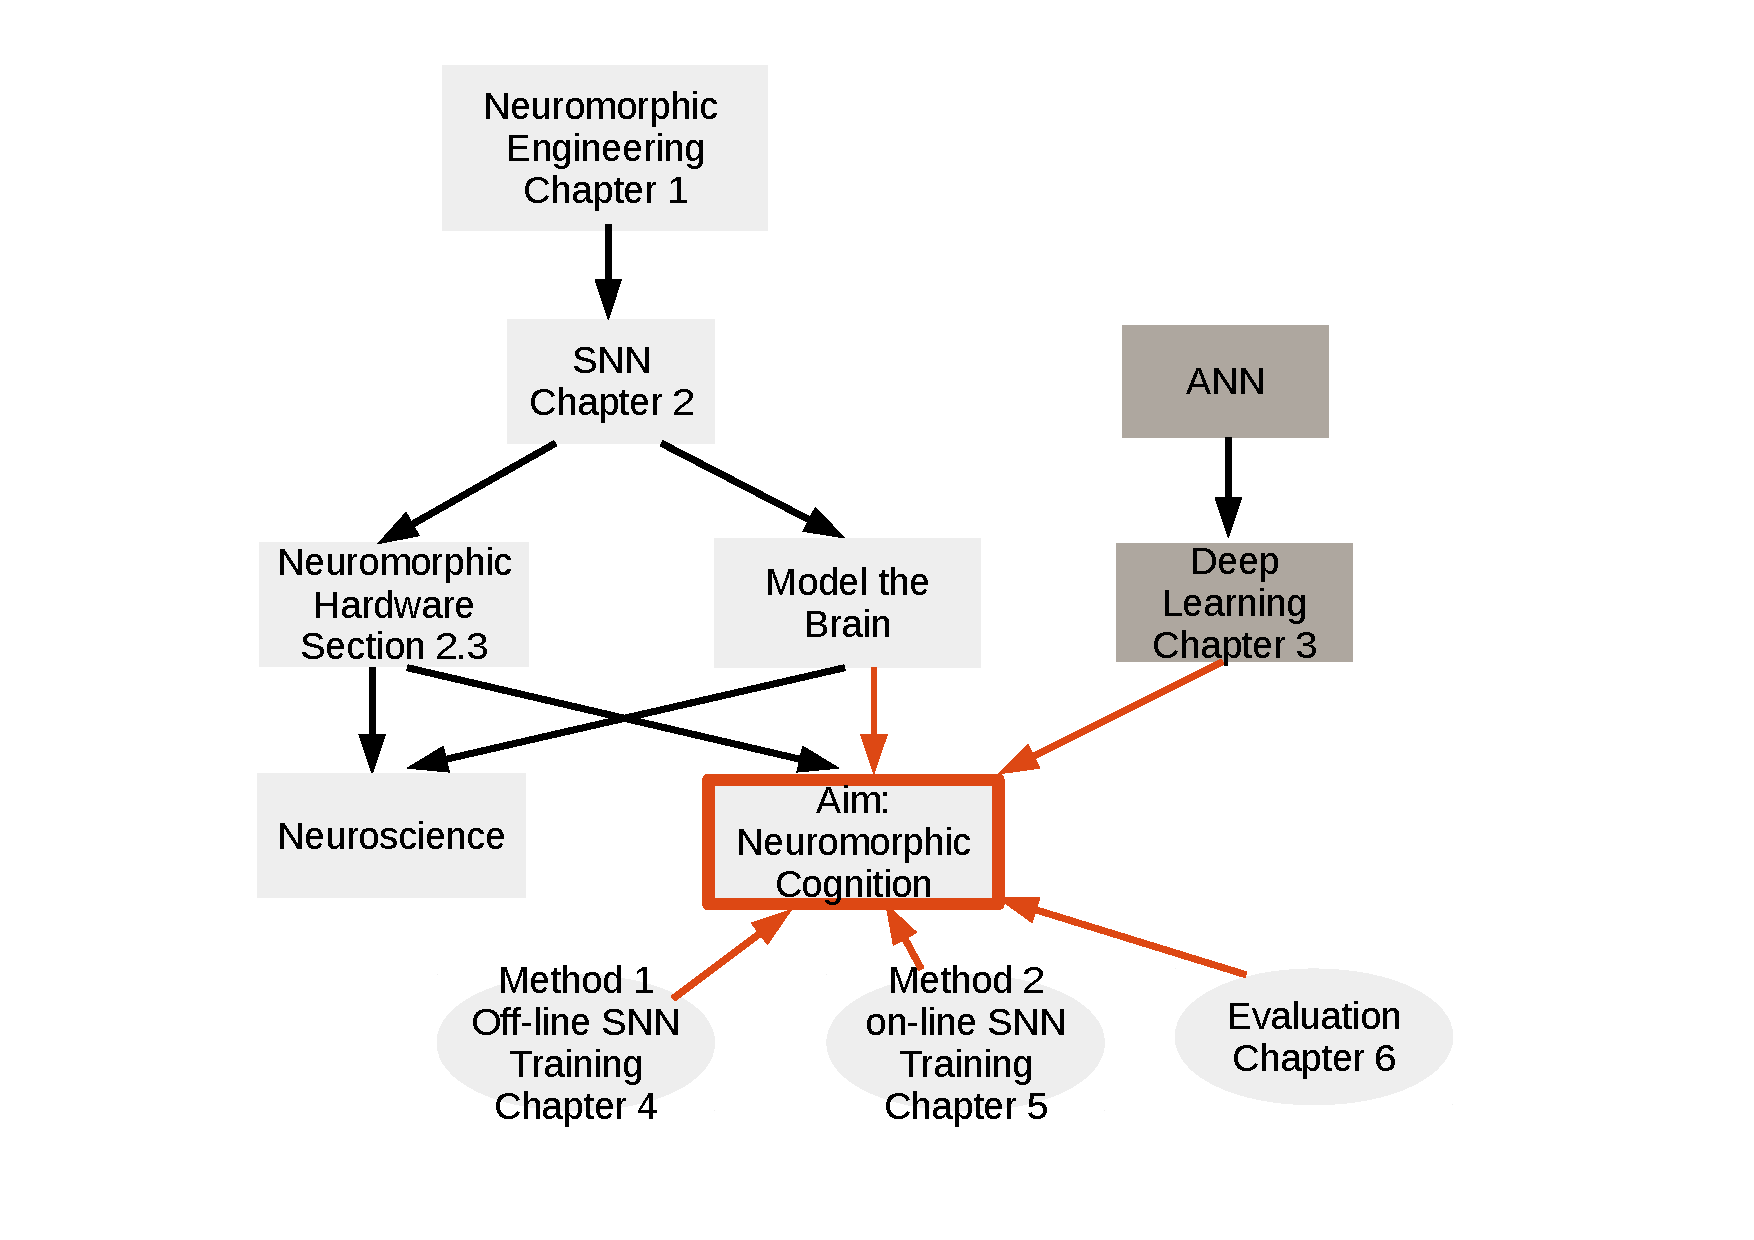
\includegraphics[width=0.95\textwidth]{pics_intro/intro_new.pdf}
		\caption{\DIFaddFL{
			The outline of the thesis.
		}}
		\label{fig:intro}
	\end{figure}

	\DIFadd{In brief, Figure~\ref{fig:intro} summarises the introduction and demonstrates the outline of the thesis.
	}

	\DIFadd{Chapter~\ref{cha:intro} introduces the aims of NE: modelling the brain, and building brain-like machines.
	Although progress has been made in both directions, it is still far from achieving the long term goal of Neuromorphic Cognition.
	With the support of accumulated knowledge of SNNs and the massive neuromorphic SNN simulators (both refer to Chapter~\ref{cha:bkg}), plus the huge success of Deep Learning in ANNs (see Chapter~\ref{cha:dnn}), the research aims at understanding how to operate and train biologically-plausible SNNs to close the gap in cognitive capabilities between SNNs and ANNs on AI tasks, thus approaching Neuromorphic Cognition.
	}

	\DIFadd{To achieve the thesis aim, we propose an on-line (Chapter~\ref{cha:Conv}) and an off-line (Chapter~\ref{cha:sdlm}) SNN training method to bring Deep Learning advantages to SNNs, and provide a spike-based dataset and its corresponding evaluation methodology to measure the performance of SNN models and their hardware implementations in Chapter~\ref{cha:bench}.
 }\DIFaddend